При большой энергии излучения поглощение фотонов электронами становится
маловероятным. Здесь при взаимодействии излучения с веществом наблюдается
рассеяние излучения.

Схематически экспериментальная установка Комптона 
изображена на рис. \ref{fig:kompton}. Рентгеновская трубка РТ была смонтирована
на вращающейся платформе, что позволяло при ее повороте 
изменять угол рассеяния $ \theta $ рентгеновского излучения, попадающего
после мишени-рассеивателя в измерительный блок установки.

\begin{figure}[h]
  \centering
  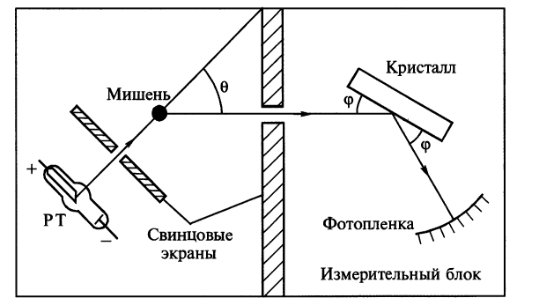
\includegraphics[width=0.8\textwidth]{img/oral-05/kompton}
  \label{fig:kompton}
\end{figure}

Длина волны рассеянного излучения определялась с помощью
дифракции его на кристалле. Согласно дифракционной теории,
при выполнении условия Брэгга -- Вульфа 
\[
    2d\sin\varphi = n\lambda', \quad n = 1,2, \ldots,
\]
где $ d $ --- расстояние между атомными плоскостями кристалла, а $ \varphi $ ---
угол скольжения падающего излучения, наблюдается 
интенсивное отражение от кристалла рассеянного рентгеновского излучения.
Поэтому, зная параметры кристаллической решетки $ d $, и измерив
угол $ \varphi $ для максимума отражения $ n $-го порядка, можно рассчитать
длину волны $ \lambda' $ рентгеновского излучения, рассеянного мишенью.
Соответствие угла $ \varphi $ и длины волны $ \lambda' $, вытекающее из формулы
выше, 
позволяло нанести на фотопленку шкалу длин волн и по положению
на фотопленке засвеченной полоски определить длину волны 
рассеянного рентгеновского излучения. В первых опытах Комптона 
вместо фотопленки использовалась подвижная ионизационная камера,
позволяющая по значению тока в приборе фиксировать отраженное
от кристалла рентгеновское излучение.

Экспериментально определено, что разность длин волн зависит только от угла $
\theta $: 
\[
    \Delta \lambda = \lambda' - \lambda = \Lambda_K (1-\cos\theta),
\]
где $ \Lambda_K = 2.426\times10^{-12} $ м.

С точки зрения классической физики этот эффект необъясним. Там рассеяние можно
рассматривать как вынужденые колебания электронов (под действием силы
электромагнитных волн), и излучение им вторичных рассеяных волн, но на той же
частоте.

В квантовой оптике этот эффект объясняется как следствие упругого рассеяния
фотона $ \Phi \to \Phi' $ на свободном электроне вещества (см. рис.
\ref{fig:compton2}). Формула Комптона тогда есть следствие законов сохранения
энергии и импульса.

\begin{figure}[H]
	\begin{center}
		\begin{tikzpicture}[thick]
			\begin{scope}
				\path [draw=blue,snake arrow,->]
				(-4,0) -- (-2,0) node[anchor=south]{\hspace{-2cm}$h\nu$};
				\filldraw[black] (-1,0) circle (2pt) node[anchor=north]{$\vec e$};
			\end{scope}
			$\implies$
			\begin{scope}
				\path [draw=blue,dashed] (1,0)--(4,0);
				\path [draw=blue,snake arrow,->]
				(2,0) -- (3.5,1) node[anchor=east]{\hspace{-2cm}$h\nu'$};
				\path [draw=black, ->]
				(2,0) -- (2.5,-1) node[anchor=west]{$\vec p_e$};
				\draw[black] (3,0) arc (0:31:1) node[anchor=west]{$\theta$};
			\end{scope}
		\end{tikzpicture}
	\end{center}
	\caption{Комптон-эффект}
  \label{fig:compton2}
\end{figure}

Действительно, $ E = h\nu = (hc)/\lambda $ и закон сохранения энергии принимает
вид
\[
    \frac{hc}{\lambda} + m_0c^2 = \frac{hc}{\lambda'} + mc^2.
\]
Здесь $ m = \gamma m_0 $, $ \gamma = (1-v^2/c^2)^{-1/2} $ --- релятивистский
множитель. Уже сейчас видно, что $ \lambda' > \lambda $.

Закон сохранения импульса принимает вид 
\[
    \hbar \mathbf k = \hbar \mathbf k' + m \mathbf v,
\]
откуда, учитывая $ k = 2\pi/\lambda $,
\[
  (mv)^2 = \left( \frac{h}{\lambda} \right)^2  + \left( \frac{h}{\lambda'}
  \right)^2 - 2 \frac{h^2}{\lambda \lambda'}\cos\theta.
\]

\begin{figure}[H]
	\begin{center}
		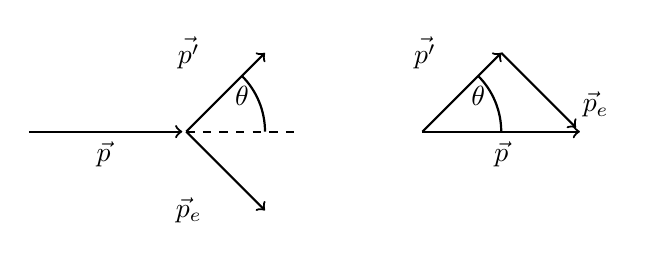
\begin{tikzpicture}[thick]
			\begin{scope}
				\path[draw=black,->] (-2,0)--(-0.05,0) node[anchor=north]{\hspace{-2cm}$\vec p$};
				\path[draw=black,->] (0,0)--(1,1) node[anchor=west]{\hspace{-2cm}$\vec {p'}$};
				\path[draw=black,->] (0,0)--(1,-1) node[anchor=west]{\hspace{-2cm}$\vec p_e$};
				\draw[black] (1,0) arc (0:45:1) node[anchor=north]{$\theta$};
				\path[draw=black,dashed] (0,0)--(1.4,0) ;
			\end{scope}
			%			$\Leftrightarrow$
			\begin{scope}
				\path[draw=black,->] (3,0)--(5,0) node[anchor=north]{\hspace{-2cm}$\vec p$};
				\path[draw=black,->] (3,0)--(4,1) node[anchor=west]{\hspace{-2cm}$\vec {p'}$};
				\path[draw=black,->] (4,1)--(4.95,0.05) node[anchor=south]{\hspace{0.5cm}$\vec p_e$};
				\draw[black] (4,0) arc (0:45:1) node[anchor=north]{$\theta$};
			\end{scope}
		\end{tikzpicture}
	\end{center}
	\caption{Закон сохранения импульса}
\end{figure}

Преобразуем теперь закон сохранения энергии к виду  
\begin{align*}
  mc &= m_0 c + \frac{h}{\lambda} - \frac{h}{\lambda'},\\
  (mc)^2 &= (m_0c)^2 + 2m_0ch \left( \frac{1}{\lambda} - \frac{1}{\lambda'}
  \right) + \left( \frac{h}{\lambda} \right)^2 - \frac{2h^2}{\lambda\lambda'} +
  \left( \frac{h}{\lambda'} \right)^2.
\end{align*}
Из соотношения $ (mc)^2 - (m_0c)^2 = (mv)^2 $ выразим соответствующим образом $
mv $ и объединим законы сохранения формулой 
\[
    2m_0 ch \left( \frac{1}{\lambda} - \frac{1}{\lambda'} \right) =
    \frac{2h^2}{\lambda\lambda'}(1-\cos\theta).
\]
Отсюда и получаем формулу Комптона  
\[
    \lambda' - \lambda = \frac{}{}
\]

